\chapter{Introduction to project}
In this project I used Raspberry Pi 4 GB. Firstly I tried to use raspi cam with raspberry, but then I get an error and never be able to fix it. Then I used web cam with raspi.

\section{Why raspi?}
Raspberry Pi boards are relatively inexpensive compared to high-end computers or dedicated hardware for object detection. This makes them an attractive option for projects with budget constraints or for hobbyists and students.\\
Raspberry Pi devices are designed to be energy-efficient, consuming significantly less power compared to traditional computers. This makes them suitable for deployment in scenarios where power consumption is a concern, such as remote or battery-powered applications. We will use it in a minibar and it would run always.
So energy-efficiency is very important for us.


\section{Minibar}
Firstly I get an old minibar. It was working but it was not in a good shape. So I painted it for my project.
It's small so it can not get more products but it's good for project.

\begin{figure}[!htbp]
    \centering
    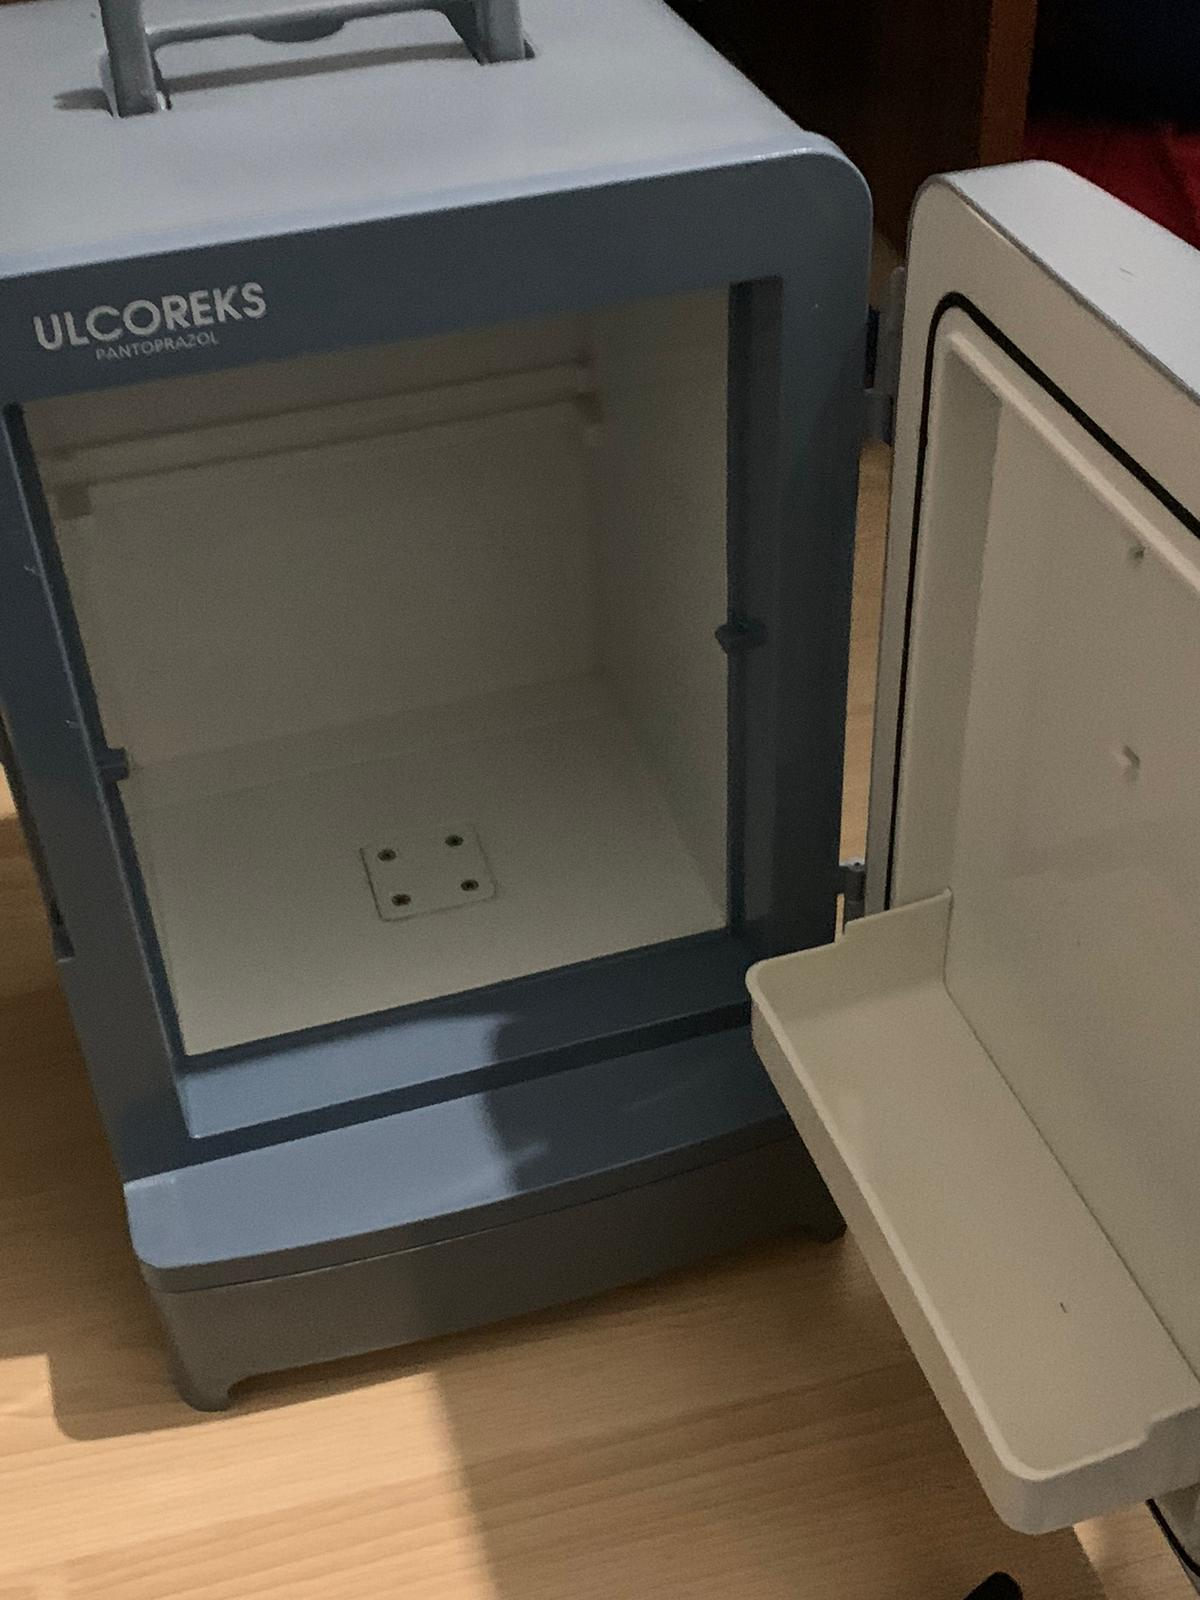
\includegraphics[width=1\textwidth]{Imgs/minibar.jpg}
    \caption{\label{fig:pic1}Minibar.}
\end{figure}

\begin{figure}[!htbp]
    \centering
    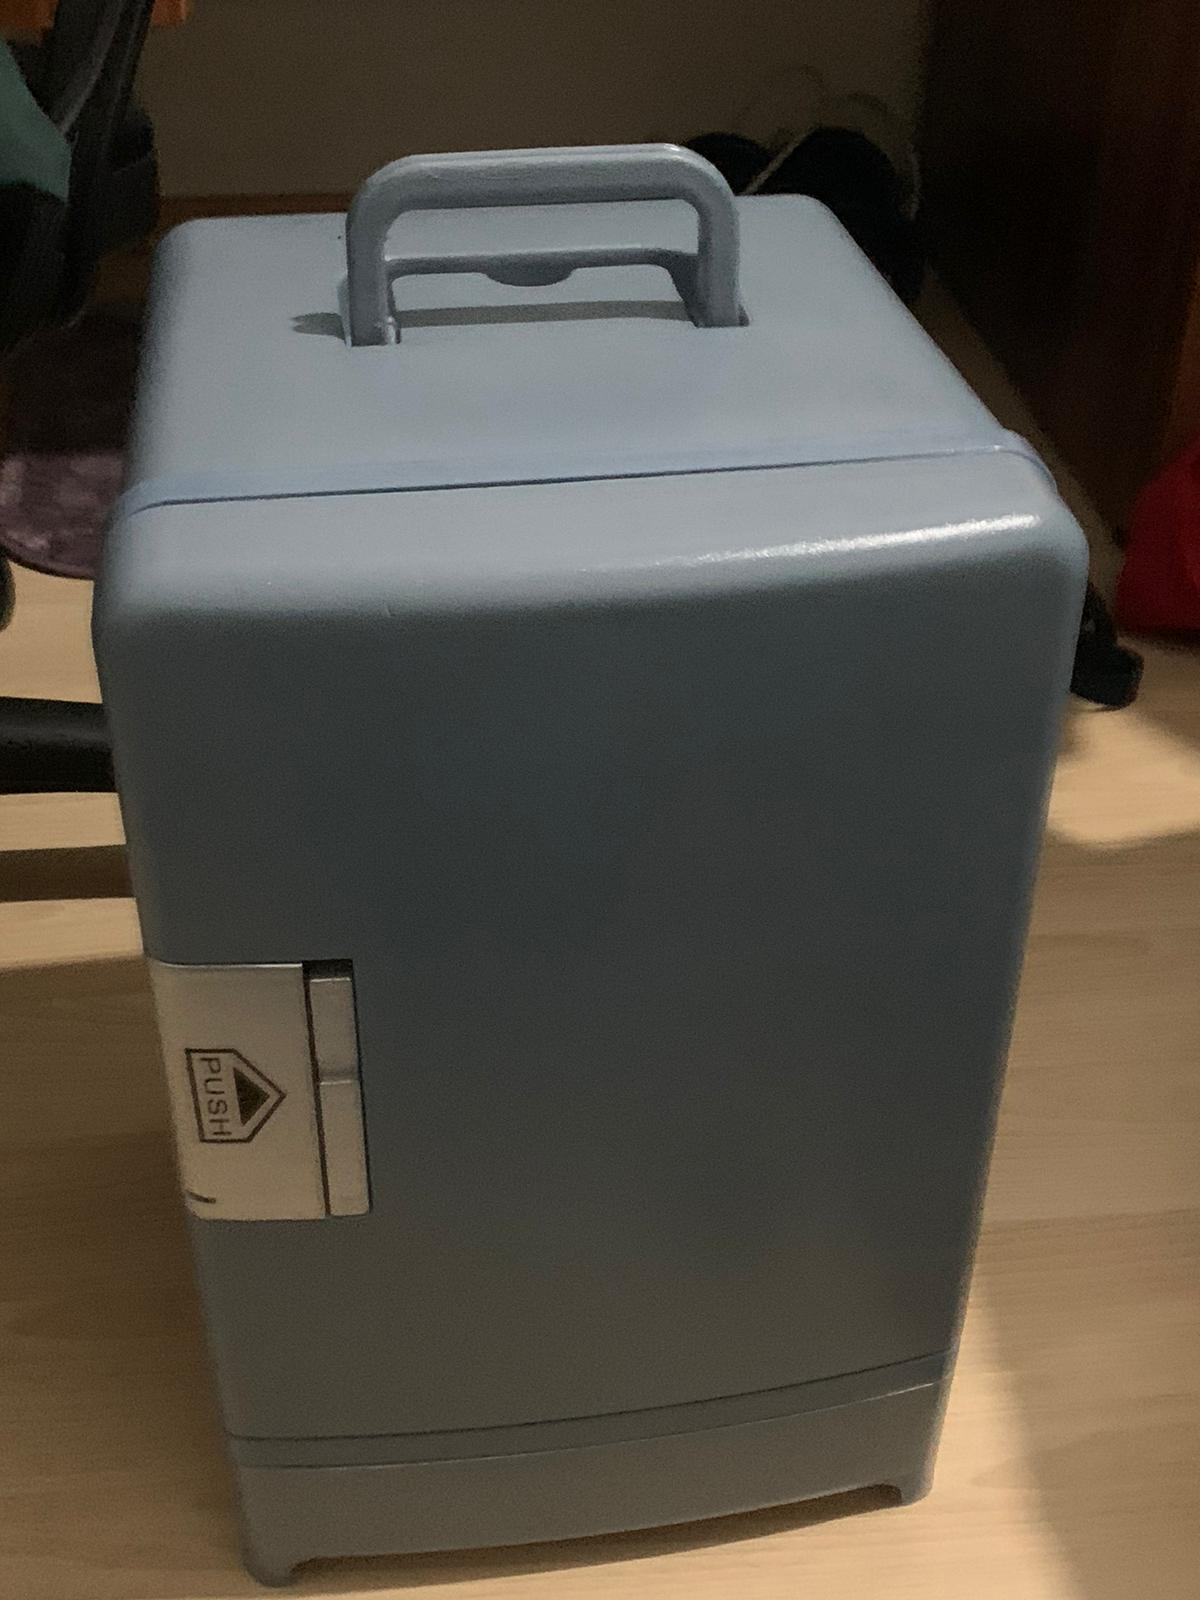
\includegraphics[width=1\textwidth]{Imgs/minibar2.jpg}
    \caption{\label{fig:pic1}Minibar.}
\end{figure}
